% Source: Wald GR, physical PDF p. 359 (printed p. 346).
% Coverage: Figure 13.1, deformation of a \(4\pi\) rotation.
% Figures/tables/footnotes: one figure asset; no tables or footnotes.
% Status: source-reviewed and compile-clean.
% Uncertainties: none.

\begingroup
\renewcommand{\thefigure}{13.1}
\begin{figure}[htbp]
  \centering
  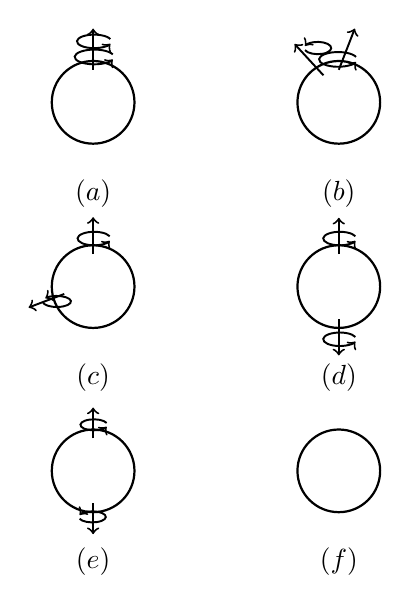
\begin{tikzpicture}[scale=.78,
      sphere/.style={draw,line width=.8pt,circle,minimum size=1.05cm},
      spin/.style={->,line width=.7pt}]
    \foreach \x/\y/\lab/\mode in {
      0/3/(a)/top,
      4/3/(b)/slant,
      0/0/(c)/side,
      4/0/(d)/double,
      0/-3/(e)/opposite,
      4/-3/(f)/none} {
      \begin{scope}[shift={(\x,\y)}]
        \node[sphere] (s) at (0,0) {};
        \ifx\mode\empty
        \fi
        \ifx\mode\relax
        \fi
        \def\top{top}\def\slant{slant}\def\side{side}\def\double{double}\def\opposite{opposite}\def\none{none}
        \ifx\mode\top
          \draw[spin] (0,.53) -- (0,1.2);
          \draw[spin] (.32,.78) arc[start angle=20,end angle=340,x radius=.32,y radius=.12];
          \draw[spin] (.28,1.03) arc[start angle=20,end angle=340,x radius=.28,y radius=.11];
        \fi
        \ifx\mode\slant
          \draw[spin] (0,.53) -- (.26,1.2);
          \draw[spin] (.28,.74) arc[start angle=20,end angle=340,x radius=.31,y radius=.12];
          \draw[spin] (-.25,.44) -- (-.72,.95);
          \draw[spin] (-.55,.85) arc[start angle=200,end angle=520,x radius=.22,y radius=.10];
        \fi
        \ifx\mode\side
          \draw[spin] (0,.53) -- (0,1.13);
          \draw[spin] (.27,.82) arc[start angle=20,end angle=340,x radius=.27,y radius=.11];
          \draw[spin] (-.47,-.12) -- (-1.05,-.34);
          \draw[spin] (-.82,-.25) arc[start angle=185,end angle=505,x radius=.23,y radius=.09];
        \fi
        \ifx\mode\double
          \draw[spin] (0,.53) -- (0,1.12);
          \draw[spin] (.27,.82) arc[start angle=20,end angle=340,x radius=.27,y radius=.11];
          \draw[spin] (0,-.53) -- (0,-1.12);
          \draw[spin] (.27,-.82) arc[start angle=20,end angle=340,x radius=.27,y radius=.11];
        \fi
        \ifx\mode\opposite
          \draw[spin] (0,.53) -- (0,1.03);
          \draw[spin] (.22,.78) arc[start angle=20,end angle=340,x radius=.22,y radius=.09];
          \draw[spin] (0,-.53) -- (0,-1.03);
          \draw[spin] (-.22,-.78) arc[start angle=200,end angle=520,x radius=.22,y radius=.09];
        \fi
        \node at (0,-1.48) {\(\lab\)};
      \end{scope}
    }
  \end{tikzpicture}
  \caption{A diagram illustrating how a rotation of a sphere by \(4\pi\) about a
  given axis can be continuously deformed to no rotation. We break up the
  \(4\pi\)-rotation into two \(2\pi\)-rotations and continuously change the axis of
  the second \(2\pi\)-rotation until it is opposite the axis of the first rotation, as
  shown in the sequence \((a)\)--\((d)\). Then we continuously decrease the angle of
  both rotations to zero, as shown in the sequence \((d)\)--\((f)\).}
  \label{fig:13.1}
\end{figure}
\endgroup
